\documentclass[11pt, oneside]{article}   	% use "amsart" instead of "article" for AMSLaTeX format
\usepackage{geometry}                		% See geometry.pdf to learn the layout options. There are lots.
\geometry{letterpaper}                   		% ... or a4paper or a5paper or ... 
%\geometry{landscape}                		% Activate for rotated page geometry
%\usepackage[parfill]{parskip}    		% Activate to begin paragraphs with an empty line rather than an indent
\usepackage{graphicx}				% Use pdf, png, jpg, or eps§ with pdflatex; use eps in DVI mode
								% TeX will automatically convert eps --> pdf in pdflatex		
\usepackage{amssymb}
\usepackage{amsmath,amssymb,amsthm,amsfonts,hyperref,fancyhdr,graphicx,subfig,bbm,multirow,array,longtable}

%SetFonts

%SetFonts

\title{Deep Learning}
\author{Bastien BRIER\\ bastien.brier@student.ecp.fr}
\date{January 5, 2017}				% Activate to display a given date or no date

\begin{document}
\maketitle
\vspace{-10pt}
\begin{center}
{\LARGE \bf Assignment 2}\\
\vspace{10pt}
\end{center}

\section{Analytic exercise}
\vspace{4pt}
	
	Given a set of training samples $\mathbf X=\{\mathbf x^1,...\mathbf x^M\}$, the log-likelihood $\mathbf X$ is:
	\[\begin{split}
		S(\mathbf X,\mathbf W)&=\sum_{m=1}^M\log P(\mathbf x^m;\mathbf W)\\
		&=\sum_{m=1}^M\log\sum_\mathbf h\frac{1}{Z}\exp(-E(\mathbf x^m,\mathbf h;\mathbf W))\\
		&=\sum_{m=1}^M\log\frac{1}{Z}\sum_\mathbf h\exp(-E(\mathbf x^m,\mathbf h;\mathbf W))\\
		&=\sum_{m=1}^M\log\sum_\mathbf h\exp(-E(\mathbf x^m,\mathbf h;\mathbf W)) - \sum_{m=1}^M\log Z
	\end{split}\]
	with
		\[E(\mathbf x,\mathbf h;\mathbf W)=E(\mathbf y;\mathbf W)=-\frac{1}{2}\mathbf y^T\mathbf W\mathbf y\:(\text{with }\mathbf y=\begin{bmatrix}  \mathbf x \\ \mathbf h \end{bmatrix})\]
		\[Z=\sum_\mathbf h\sum_\mathbf x\exp(-E(\mathbf x,\mathbf h;\mathbf W)) = \sum_\mathbf y\exp(-E(\mathbf y;\mathbf W))\]	
	As derivation is linear, we can compute the derivative of the first part of the equation and then the second, so:
	\[\begin{split}
		\frac{\partial \log\sum_\mathbf h\exp(-E(\mathbf x^m,\mathbf h;\mathbf W))}{\partial w_{k,l}}&=\frac{1}{\sum_\mathbf h\exp(-E(\mathbf x^m,\mathbf h;\mathbf W))}\times \frac{\partial \sum_\mathbf h\exp(-E(\mathbf x^m,\mathbf h;\mathbf W))}{\partial w_{k,l}}\\
		&=\frac{1}{\sum_\mathbf h\exp(-E(\mathbf x^m,\mathbf h;\mathbf W))}\times \sum_\mathbf h \frac{\partial \exp(-E(\mathbf x^m,\mathbf h;\mathbf W))}{\partial w_{k,l}}\\
		&=\frac{1}{\sum_\mathbf h\exp(-E(\mathbf x^m,\mathbf h;\mathbf W))}\times \sum_\mathbf h \exp(-E(\mathbf x^m,\mathbf h;\mathbf W))\times \frac{\partial (-E(\mathbf x^m,\mathbf h;\mathbf W))}{\partial w_{k,l}}\\
		&=\frac{\sum_\mathbf h\mathbf y_{k}\mathbf y_{l}\exp(-E(\mathbf x^m,\mathbf h;\mathbf W))}{\sum_\mathbf h\exp(-E(\mathbf x^m,\mathbf h;\mathbf W))}\\
	\end{split}\]
	Moreover, we know that:
	\[P(\mathbf h | \mathbf x^m;\mathbf W) = \frac{\exp(-E(\mathbf x^m,\mathbf h;\mathbf W))}{\sum_\mathbf h\exp(-E(\mathbf x^m,\mathbf h;\mathbf W))}\]
	Then:
	\[\begin{split}
		\frac{\partial \log\sum_\mathbf h\exp(-E(\mathbf x^m,\mathbf h;\mathbf W))}{\partial w_{k,l}}&=\sum_\mathbf h \mathbf y_{k}\mathbf y_{l} P(\mathbf h | \mathbf x^m;\mathbf W)\\
		&=\langle \mathbf y_{k} \mathbf y_{l}\rangle_{P(\mathbf h,\mathbf x^m;\mathbf W)}
	\end{split}\]
	We compute the derivation of the second part of the equation:
	\[\begin{split}
		\frac{\partial \log Z}{\partial w_{k,l}}&=\frac{1}{Z}\times \frac{\partial \sum_{\mathbf h, \mathbf x}\exp(-E(\mathbf x, \mathbf h; \mathbf W))}{\partial w_{k,l}}\\
		&=\frac{1}{Z}\sum_{\mathbf h, \mathbf x}\frac{\partial \exp(-E(\mathbf x, \mathbf h; \mathbf W))}{\partial w_{k,l}}\\
		&=\frac{1}{Z}\sum_{\mathbf h, \mathbf x}\frac{\partial(-E(\mathbf x, \mathbf h; \mathbf W))}{\partial w_{k,l}}\times \exp(-E(\mathbf x, \mathbf h; \mathbf W))\\
		&=\frac{1}{Z}\sum_{\mathbf h, \mathbf x}\mathbf y_{k}\mathbf y_{l}\exp(-E(\mathbf x, \mathbf h; \mathbf W))\\
		&=\frac{1}{Z}\sum_{\mathbf y}\mathbf y_{k}\mathbf y_{l}\exp(-E(\mathbf y; \mathbf W))
	\end{split}\]
	We know that:
	\[P(\mathbf y;\mathbf W) = \frac{1}{Z}\exp(-E(\mathbf y; \mathbf W))\]
	Therefore:
	\[\begin{split}
		\frac{\partial \log Z}{\partial w_{k,l}}&=\sum_{\mathbf y}\mathbf y_{k}\mathbf y_{l}P(\mathbf y;\mathbf W)\\
		&=\sum_{\mathbf h, \mathbf x}\mathbf y_{k}\mathbf y_{l}P(\mathbf h,\mathbf x;\mathbf W)\\
		&=\langle \mathbf y_{k} \mathbf y_{l}\rangle_{P(\mathbf h,\mathbf x;\mathbf W)}
	\end{split}\]
	Putting it all together:
	\[\begin{split}
		\frac{\partial S(\mathbf X, \mathbf W)}{\partial w_{k,l}}&=\sum_{m=1}^M\langle \mathbf y_{k} \mathbf y_{l}\rangle_{P(\mathbf h,\mathbf x^m;\mathbf W)} - \sum_{m=1}^M\langle \mathbf y_{k} \mathbf y_{l}\rangle_{P(\mathbf h,\mathbf x;\mathbf W)}\\
		&=\sum_{m=1}^M[\langle \mathbf y_{k} \mathbf y_{l}\rangle_{P(\mathbf h,\mathbf x^m;\mathbf W)} - \langle \mathbf y_{k} \mathbf y_{l}\rangle_{P(\mathbf h,\mathbf x;\mathbf W)}]
	\end{split}\]

\section{Exact summations}
\vspace{4pt}

	We use brute-force summations to obtain the exact value of the log-likelihood for three models : Ising Model, Boltzmann Machine and Restricted Boltzmann Machine.\\
	We implemented gradient-ascent and here are the plots obtained.\\

	\begin{figure}[h]
		\centering
		\caption{Brute-force summation, 8 hidden layers}
		\begin{tabular}[h]{cc}
			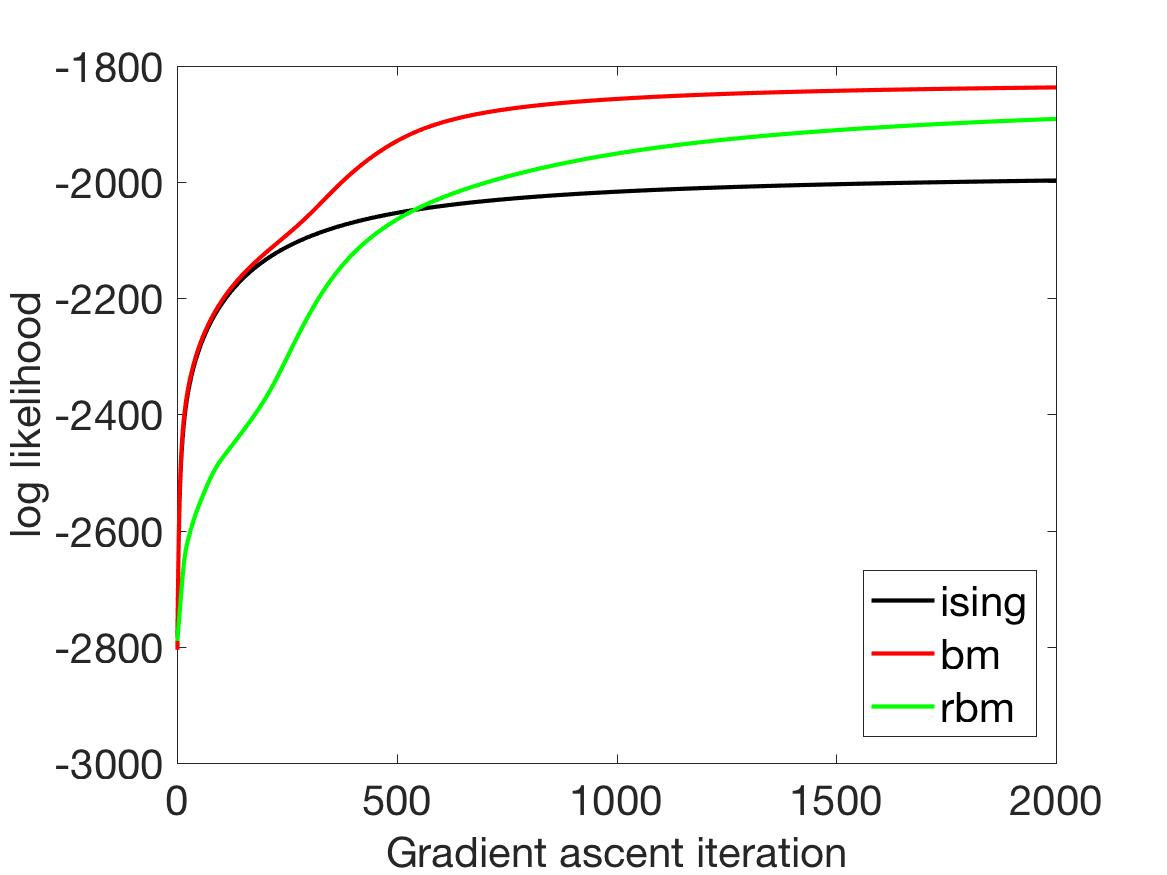
\includegraphics[width=8cm]{/Users/bastienbrier/Pictures/log_likelihood_brute_force_nhidden_8.jpg}
			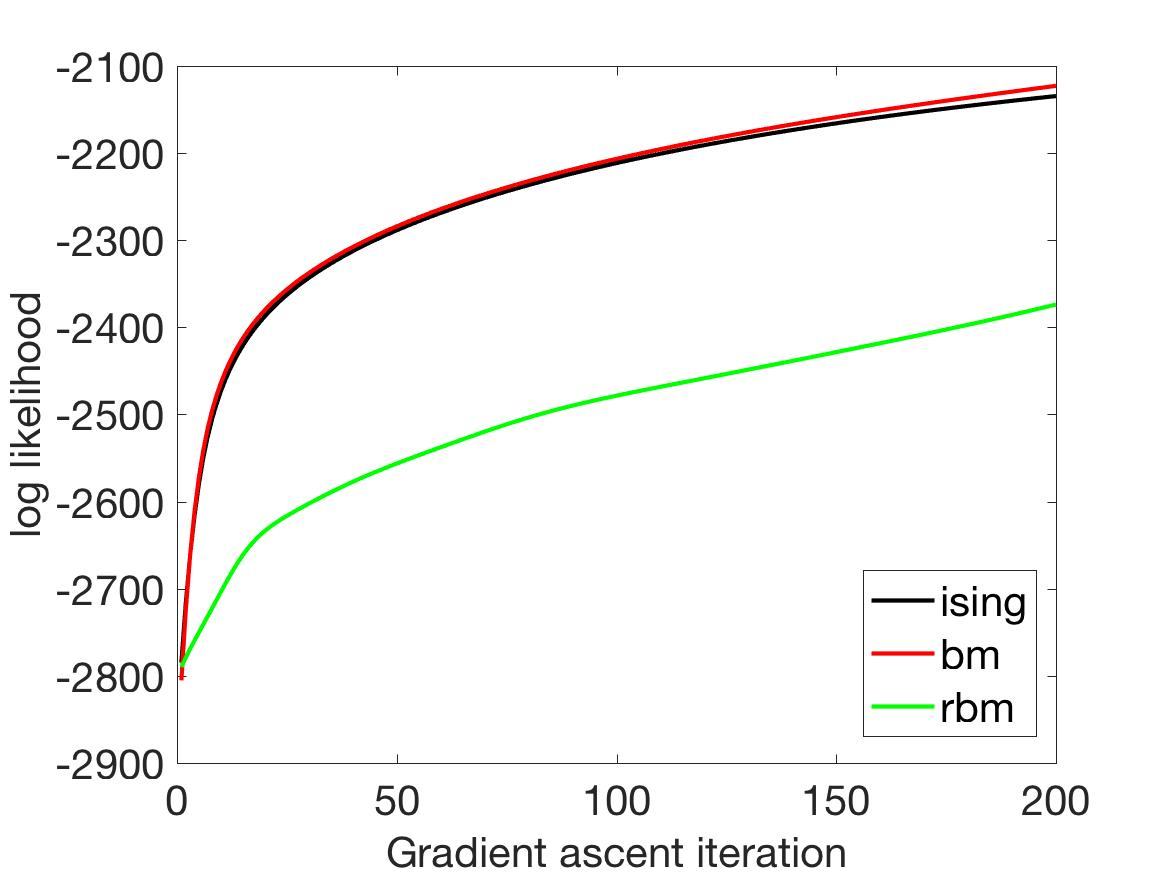
\includegraphics[width=8cm]{/Users/bastienbrier/Pictures/log_likelihood_brute_force_nhidden_8_200.jpg}
		\end{tabular}
	\end{figure}	
	
	As expected, the best performance is reached by the full Boltzmann machine, as it is fully connected between observable and hidden layers. As the first estimations are based on the observable variables, the Ising model and Boltzmann Machine perform way better than the Restricted BM in the right plot. But then, the hidden layers improve the accuracy of the summation and, from the 500th iteration, the Restricted Boltzmann Machine has better performance than the Ising Model. In the end, the performance of the BM and RBM are better than the Ising Model.
	
\section{Block-Gibbs sampling and Contrastive Divergence}
\vspace{4pt}

	After having implemented Block-Gibbs sampling, we used contrastive divergence with L = 1 and L = 10 to train a Restricted Boltzmann Machine with 8 hidden layers. Here are the plots obtained.\\
	\begin{figure}[h]
		\centering
		\caption{Contrastive Divergence, 8 hidden layers}
		\begin{tabular}[h]{cc}
			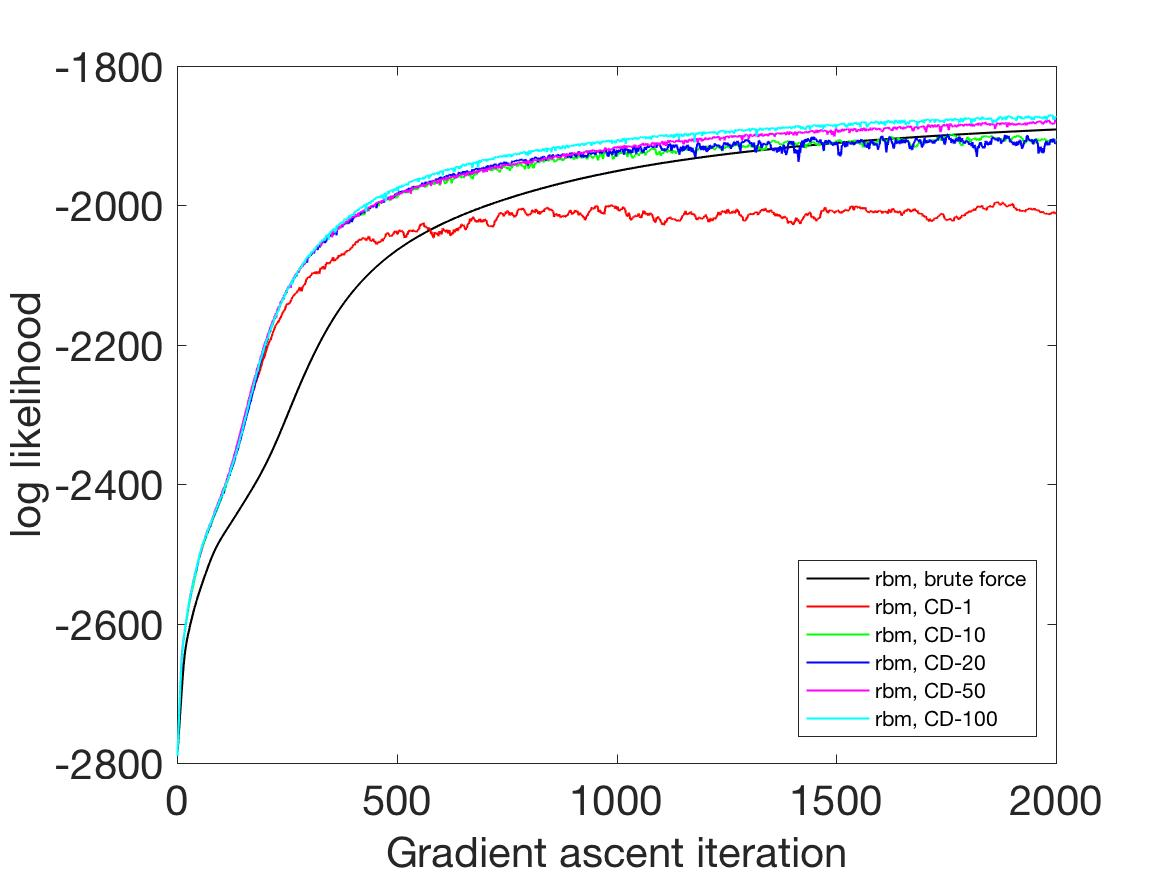
\includegraphics[width=8cm]{/Users/bastienbrier/Pictures/log_likelihood_monte_carlo_nhidden_8.jpg}
			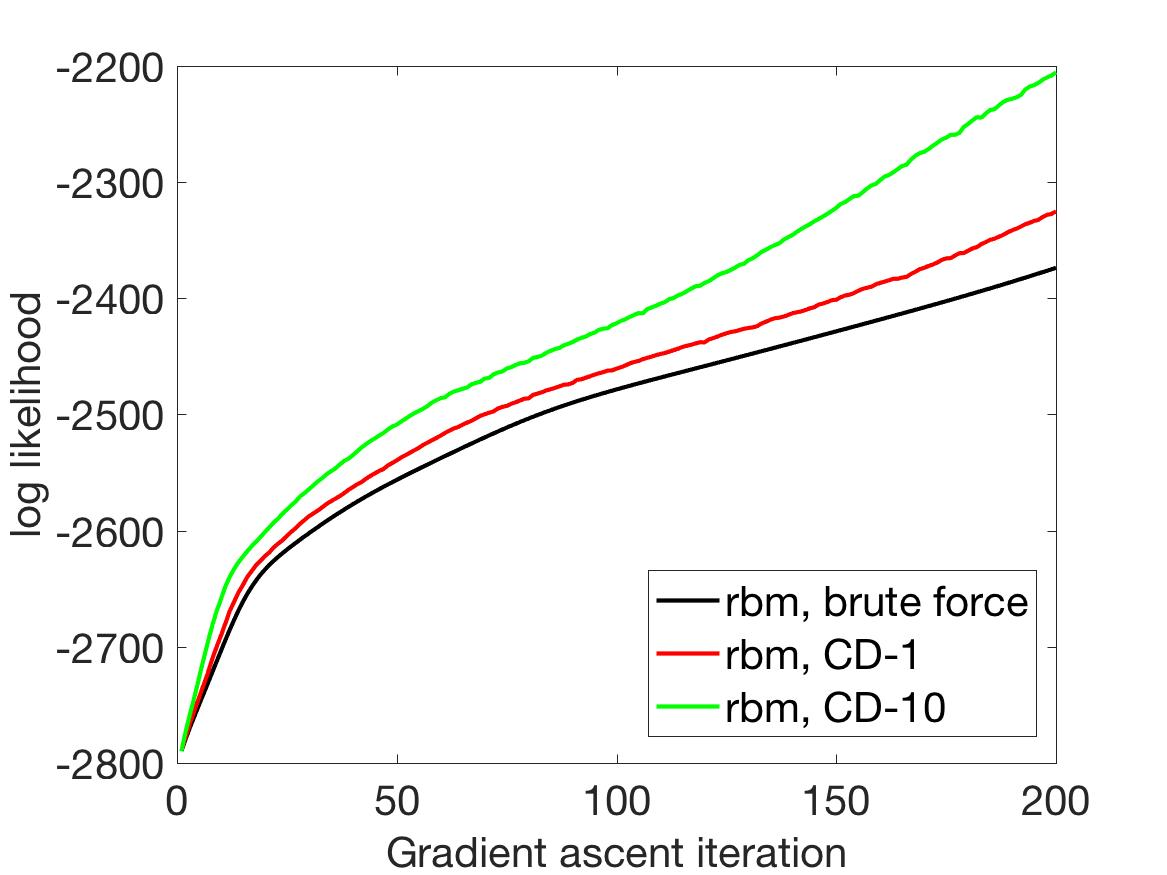
\includegraphics[width=8cm]{/Users/bastienbrier/Pictures/log_likelihood_monte_carlo_nhidden_8_200.jpg}
		\end{tabular}
	\end{figure}
	
	As expected, after 2000 iterations, the best result is obtained by the brute-force summation. But, the CD approximations have better results in the beginning.  The principle of Gibbs sampling is that we condition x (visible) and sample h, and then condition h and sample x, L times. Is is then not surprising that the CD with L=10 has better results than the one with L=1. For 2000 iterations, the result of the CD with L=10 is really close to the brute-force summation.
	
\end{document}  